%
% Qualitative example of switch bouncing versus CPU clock.
%
\documentclass[border=3mm]{standalone}
\usepackage{tikz}
\usetikzlibrary{circuits.ee.IEC}

\begin{document}

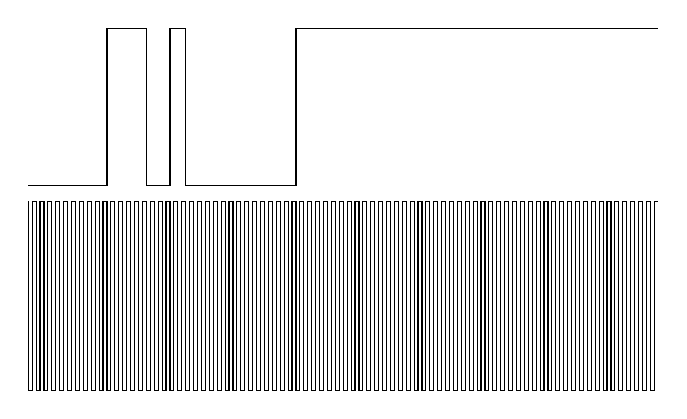
\begin{tikzpicture}
    \draw [-] (0,0)
        to (1.0,0) to (1.0,2)
        to (1.5,2) to (1.5,0)
        to (1.8,0) to (1.8,2)
        to (2.0,2) to (2.0,0)
        to (3.4,0) to (3.4,2)
        to (8,2);
    \foreach \x [evaluate=\x as \inieval using 2*\x] in {0,0.05,...,4}
        \draw[thin] (\inieval,-0.2) -- ++(0,-2.4) -| (\inieval+0.05,-0.2) -- (\inieval+0.1,-0.2);
\end{tikzpicture}

\end{document}

